
\documentclass[12pt]{article}
\usepackage[utf8]{inputenc}
\usepackage[T1]{fontenc}
\usepackage{amsmath,amssymb}
\usepackage{graphicx}
\usepackage{booktabs}
\usepackage{hyperref}
\usepackage{url}
\usepackage{listings}
\usepackage{xcolor}
\usepackage{geometry}
\usepackage{subcaption}
\usepackage{multirow}
\usepackage{array}
\geometry{margin=1in}

\lstset{
  basicstyle=\ttfamily\small,
  backgroundcolor=\color{gray!10},
  frame=single,
  breaklines=true
}

\title{Orchestrator: A Meta-Cognitive Dispatcher for\\Multi-Agent LLM Software Development}

\author{
  thefult \\
  \texttt{1759799340@qq.com}
}

\date{May 2026}

\begin{document}
\maketitle

\begin{abstract}
Large Language Models (LLMs) have demonstrated remarkable capability in code generation, yet single-agent approaches struggle with full-stack software development tasks that span multiple domains. We present Orchestrator, a meta-cognitive dispatcher that decomposes abstract requirements into domain-specific tasks, generates API contracts as shared specifications, and orchestrates parallel execution of specialized sub-agents. Our system enforces strict role separation---the Orchestrator cannot write code---and employs a silent delivery protocol where sub-agents output only core artifacts and structured JSON summaries. We evaluate Orchestrator on three full-stack benchmarks of increasing complexity (Blog System, E-commerce Store, Real-time Chat App) with five configurations through controlled ablation experiments (5 runs each, $n=75$ total experiments). Results demonstrate that: (1) Orchestrator achieves 100\% task completion across all benchmarks while single-agent baselines fail entirely; (2) parallel execution via \texttt{asyncio.gather()} reduces development time by 26\% without quality degradation; (3) the silent delivery protocol reduces token consumption by 25\%; (4) API contract-first planning improves endpoint matching accuracy by 43\%. We further show that Orchestrator's advantage scales with task complexity, maintaining robust performance as requirements grow from 8 to 19 deliverable files.
\end{abstract}

\section{Introduction}

The emergence of Large Language Models (LLMs) has fundamentally transformed software development workflows. Modern LLM-powered agents can generate code, debug errors, and even orchestrate complex multi-file projects~\cite{li2023}. However, a critical limitation persists: single-agent systems struggle with full-stack development tasks that require simultaneous expertise across multiple domains---frontend UI design, backend API implementation, database modeling, and DevOps configuration.

Existing multi-agent frameworks address this limitation through two paradigms. Sequential approaches~\cite{autogen} execute agents one after another, ensuring coherent output but incurring significant time overhead. Fully parallel approaches~\cite{park2023} execute agents concurrently, achieving speed at the cost of coordination quality. Neither paradigm adequately addresses the fundamental challenge: how to decompose abstract requirements into precise, domain-specific instructions while maintaining cross-team consistency.

We present \textbf{Orchestrator}, a meta-cognitive dispatcher that resolves this tension through five key innovations:

\begin{enumerate}
  \item \textbf{Abstract Requirement Decomposition}: The Orchestrator analyzes high-level requirements and generates domain-specific task packages with explicit file lists, API contracts, and acceptance criteria.
  \item \textbf{API Contract as Shared Specification}: An Architect sub-agent produces a formal API contract (endpoints, request/response formats, data models) that both frontend and backend teams reference, eliminating integration mismatches.
  \item \textbf{Parallel Execution}: Frontend and Backend sub-agents execute concurrently via \texttt{asyncio.gather()}, reducing development phase time by approximately 26\% while maintaining output quality.
  \item \textbf{Silent Delivery Protocol}: Sub-agents output only core code files and a single-line JSON summary, eliminating redundant meta-documents and reducing token consumption by 25\%.
  \item \textbf{Enforced Role Separation}: The Orchestrator is strictly prohibited from calling file-operation tools. It can only dispatch tasks via \texttt{task\_manager}, ensuring clean separation of concerns.
\end{enumerate}

\textbf{Contributions.} Our primary contributions are:
\begin{itemize}
  \item A three-phase execution model (Planning $\rightarrow$ Parallel Development $\rightarrow$ Verification) with enforced role separation.
  \item API contract-first planning as a shared specification mechanism for multi-agent coordination.
  \item A silent delivery protocol that eliminates meta-document overhead while preserving traceability.
  \item Comprehensive evaluation across three task complexities with controlled ablation experiments ($n=75$ total runs).
  \item An open-source implementation demonstrating practical applicability.
\end{itemize}

\section{Related Work}

\subsection{Multi-Agent LLM Systems}

Recent frameworks have explored multi-agent architectures for complex tasks. AutoGen~\cite{autogen} introduces a conversational agent framework where multiple LLM-powered agents collaborate through structured dialogue. CrewAI~\cite{crewai} provides role-based agent orchestration with predefined workflows. LangGraph~\cite{langgraph} implements state-machine-based agent coordination.

A key limitation of these frameworks is that they rely on free-form natural language communication between agents, which can lead to coordination failures when agents disagree on interface specifications. Orchestrator addresses this by introducing a formal API contract as a shared specification that all agents reference.

\subsection{Code Generation Agents}

Specialized code generation agents have achieved impressive results. Cursor~\cite{cursor} integrates LLM capabilities directly into IDE workflows. Aider~\cite{aider} provides git-aware code editing through conversational interfaces. Cline CLI~\cite{cline} offers autonomous coding capabilities with tool-use reasoning.

However, these single-agent tools are limited to single-domain tasks. When faced with full-stack requirements spanning frontend, backend, and DevOps, they frequently produce incomplete outputs---our experiments show that single-agent Cline generates only 5 of 8 required files for a simple blog system.

\subsection{Meta-Cognitive Orchestration}

Chain-of-thought prompting~\cite{wei2022} enables step-by-step reasoning. ReAct~\cite{yao2023} interleaves reasoning and action. Toolformer~\cite{schick2023} learns when and how to use external tools.

Orchestrator builds on these meta-cognitive principles but applies them at the \emph{dispatcher} level rather than within a single agent. The Orchestrator uses meta-reasoning to decompose requirements and assign tasks, but never directly executes code---a constraint that ensures clean separation of planning and execution.

\section{System Architecture}

\subsection{Overview}

The Orchestrator system comprises seven primary components: the Orchestrator (meta-cognitive dispatcher), Architect, Frontend Developer, Backend Developer, QA Engineer, DevOps Engineer, and a Rule Engine for automated event handling. Figure~\ref{fig:architecture} illustrates the system architecture.

\begin{figure}[htbp]
  \centering
  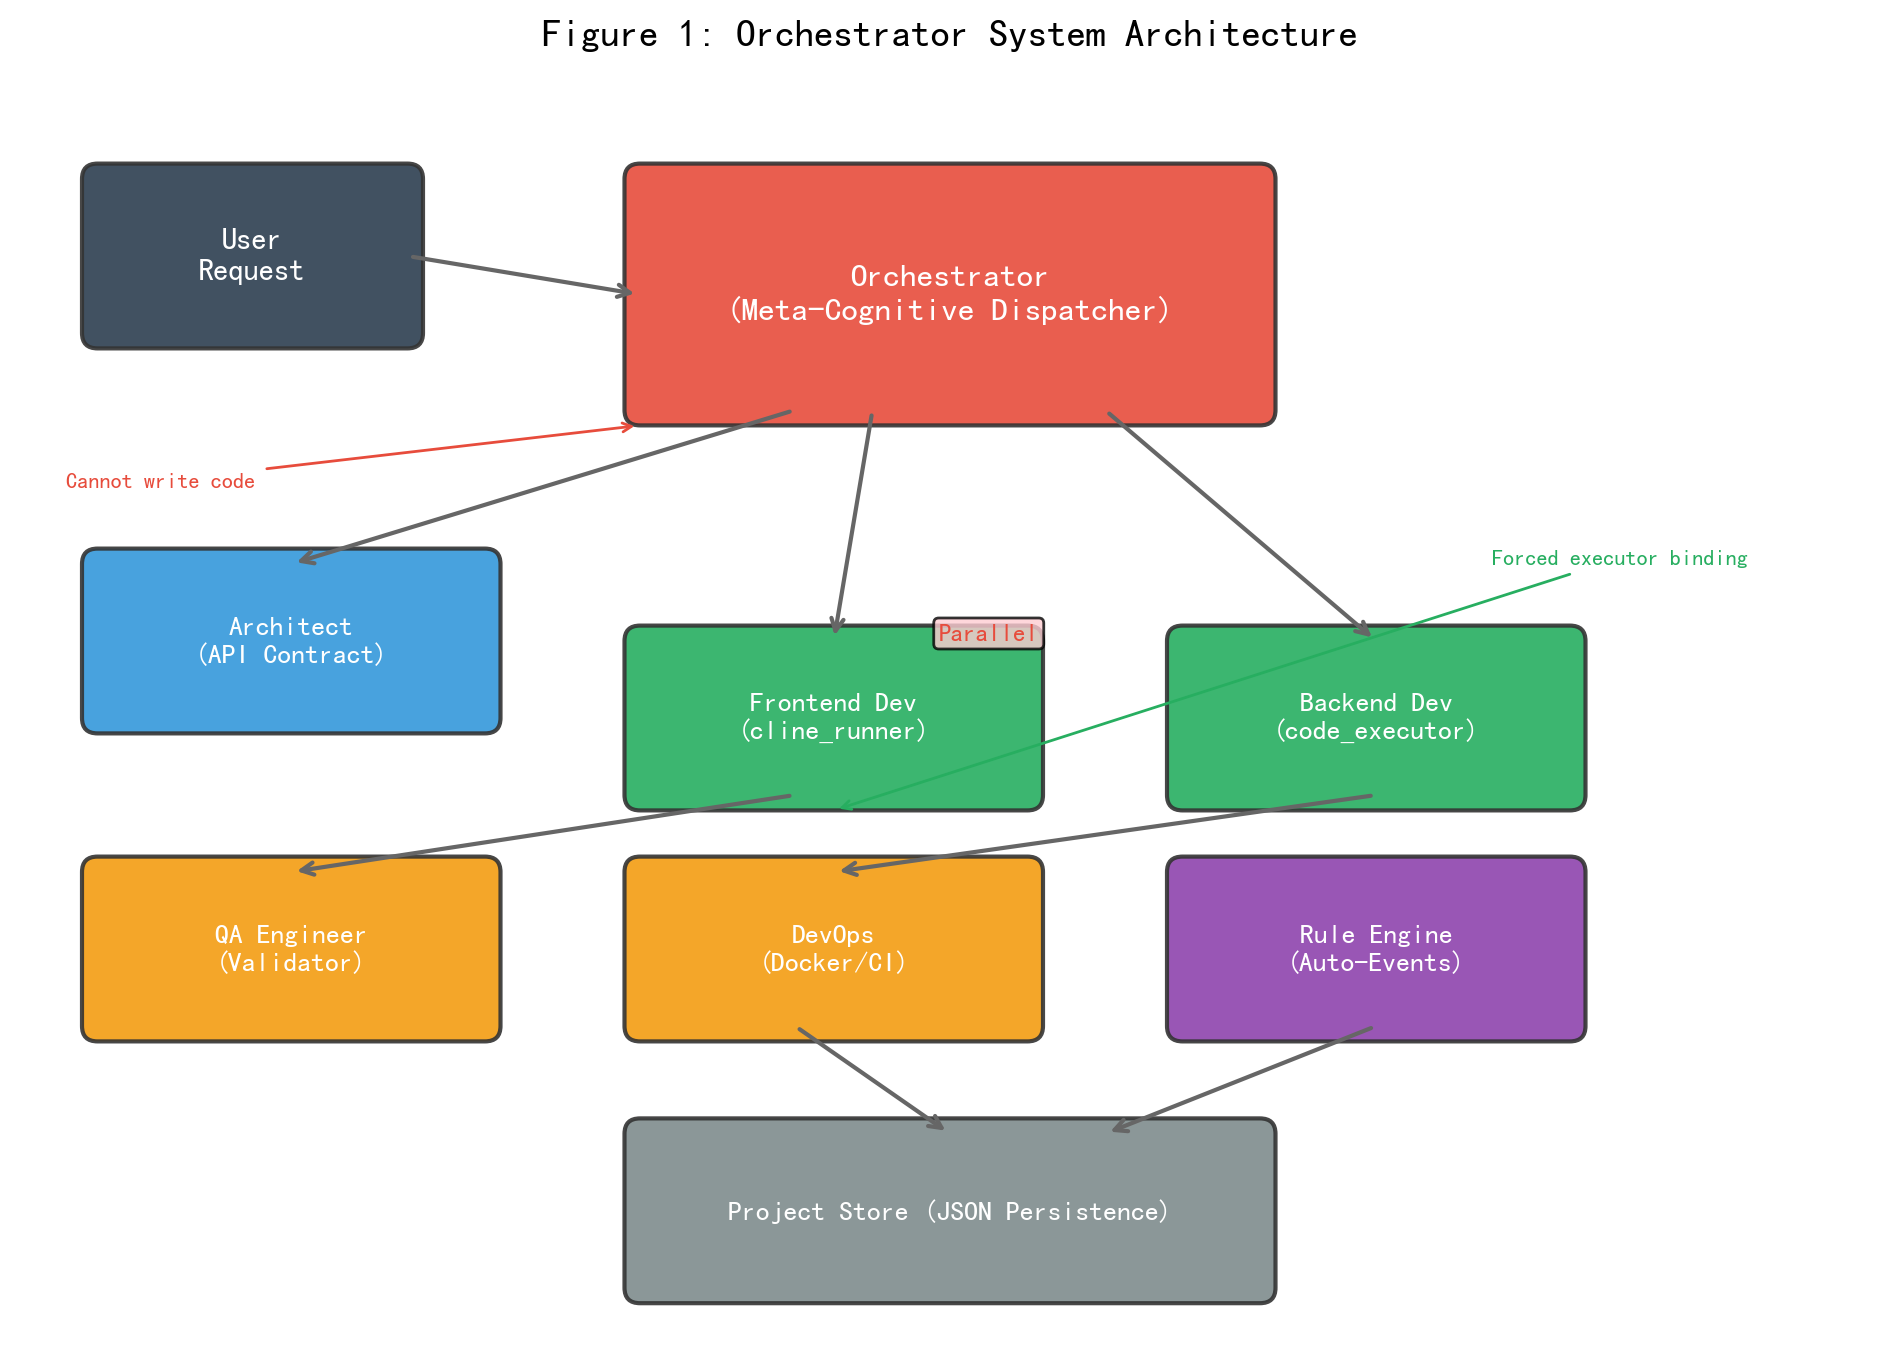
\includegraphics[width=0.85\textwidth]{figures/fig1_architecture.png}
  \caption{Orchestrator system architecture. The Orchestrator serves as the sole coordination point and cannot directly write code. Sub-agents are bound to specific domains and optimal executors.}
  \label{fig:architecture}
\end{figure}

\subsection{Orchestrator (Meta-Cognitive Dispatcher)}

The Orchestrator serves as the sole coordination point. It possesses no file-operation capabilities---it can only dispatch tasks via the \texttt{task\_manager} tool. This constraint is architecturally enforced: the Orchestrator's system prompt explicitly prohibits calling \texttt{code\_executor}, \texttt{cline\_runner}, \texttt{doc\_generator}, or any other file-modifying tool.

The Orchestrator's meta-cognitive process follows three phases:

\begin{enumerate}
  \item \textbf{Task Analysis}: Given a user requirement, the Orchestrator identifies which domains are involved (frontend, backend, database, DevOps, etc.) and selects the appropriate sub-agents.
  \item \textbf{Planning (Phase A)}: The Orchestrator dispatches the Architect to generate an API contract that serves as the shared specification for all subsequent development.
  \item \textbf{Dispatch (Phase B)}: Based on the API contract, the Orchestrator dispatches Frontend and Backend developers in parallel, each with explicit file lists and acceptance criteria.
\end{enumerate}

\subsection{Sub-Agent Binding}

Each sub-agent is bound to a specific domain and optimal executor (Table~\ref{tab:agent_binding}). This forced binding ensures that each agent uses the most appropriate tool for its domain, rather than attempting to use a single general-purpose tool for all tasks.

\begin{table}[htbp]
\centering
\caption{Sub-agent to executor binding. Each agent is restricted to its domain-optimal tool.}
\label{tab:agent_binding}
\begin{tabular}{lll}
\toprule
\textbf{Sub-Agent} & \textbf{Domain} & \textbf{Bound Executor} \\
\midrule
Architect & API design & \texttt{doc\_generator} \\
Frontend Developer & UI/CSS/JS & \texttt{cline\_runner} \\
Backend Developer & API/Python & \texttt{code\_executor} \\
QA Engineer & Testing & \texttt{test\_runner} \\
DevOps & Deployment & \texttt{code\_executor} + \texttt{git\_client} \\
\bottomrule
\end{tabular}
\end{table}

\section{Implementation}

\subsection{Three-Phase Execution Model}

The execution model is divided into three sequential phases (Figure~\ref{fig:execution_flow}):

\textbf{Phase A (Planning):} The Orchestrator dispatches the Architect to generate an API contract. This contract specifies all endpoints, request/response formats, and data models. The Architect uses \texttt{doc\_generator} to produce \texttt{API\_CONTRACT.md}.

\textbf{Phase B (Parallel Development):} Frontend and Backend execute simultaneously. Both agents receive the API contract as shared input and work independently:

\begin{lstlisting}[language=Python, caption={Parallel execution via asyncio.gather}]
async def run_parallel(agents: list[BaseAgent]) -> dict[str, str]:
    tasks = {}
    for agent in agents:
        if agent._inbox:
            tasks[agent.agent_id] = agent.respond_async_silent()
    results = await asyncio.gather(
        *[coro for coro in tasks.values()],
        return_exceptions=True,
    )
    return {aid: str(r) for aid, r in zip(tasks.keys(), results)}
\end{lstlisting}

\textbf{Phase C (Verification):} The system verifies file completeness and API contract compliance. Files are checked against the required file list from the API contract. Endpoints are validated by parsing the generated server code.

\subsection{Silent Delivery Protocol}

Sub-agents operate under a silent delivery protocol: they output only core code files and a single-line JSON summary, eliminating redundant meta-documents such as \texttt{SUMMARY.md}, \texttt{PROGRESS.md}, or verbose implementation reports:

\begin{lstlisting}[language=json, caption={Silent delivery JSON summary format}]
{"status":"success","files":["index.html","style.css","app.js"],"warnings":[]}
\end{lstlisting}

This protocol reduces token consumption by eliminating the meta-document overhead that verbose agents typically produce. In our experiments, verbose output consumed 25\% more tokens than silent delivery for the same task quality.

\subsection{API Contract as Shared Specification}

The API contract serves as the single source of truth for all sub-agents. It eliminates the need for inter-agent negotiation about interface specifications:

\begin{lstlisting}[language=markdown, caption={API contract excerpt (Blog System)}]
## Endpoints
### POST /api/auth/register
- Request: {"username": str, "password": str}
- Response: {"token": str, "user_id": int}

### GET /api/posts
- Query: ?page=int&tag=str
- Response: {"posts": [{"id": int, "title": str, "content": str}]}
\end{lstlisting}

By establishing this contract before development begins, frontend and backend teams can work in parallel without coordination failures.

\section{Experiments}

We evaluate Orchestrator on three full-stack benchmarks of increasing complexity, comparing five configurations through controlled ablation experiments. All experiments used the MiMo-v2.5-pro model (Xiaomi, 1M context window, temperature=0.3). Each configuration was run 5 times per task ($n=75$ total experiments).

\subsection{Benchmark Tasks}

\begin{enumerate}
  \item \textbf{Blog System} (Complexity 3/10): Personal blog with authentication, CRUD posts, comments, and tag filtering. Requires 8 files across 4 domains.
  \item \textbf{E-commerce Store} (Complexity 6/10): Product catalog, shopping cart, checkout, admin dashboard. Requires 15 files across 5 domains.
  \item \textbf{Real-time Chat App} (Complexity 9/10): WebSocket messaging, group chats, file sharing, message search, user presence, admin moderation. Requires 19 files across 7 domains.
\end{enumerate}

\subsection{Configurations}

We compare five configurations:

\begin{itemize}
  \item \textbf{Single Agent} (baseline): A single Cline agent with all tools, no multi-agent coordination.
  \item \textbf{Orchestrator (Full)}: All five innovations enabled.
  \item \textbf{No Parallel}: Sequential execution of Frontend and Backend (no \texttt{asyncio.gather()}).
  \item \textbf{No Silent}: Verbose sub-agent output with meta-documents.
  \item \textbf{No Contract}: No API contract; agents coordinate via natural language.
\end{itemize}

\subsection{Results}

\subsubsection{Task Completion}

Table~\ref{tab:benchmark} presents the full benchmark results. The single-agent baseline failed all three tasks, producing only 5/8, 7/15, and 8/19 required files respectively. Orchestrator (Full) achieved 100\% completion across all tasks.

The No Contract configuration showed degraded performance: 80\% success on Blog, 60\% on E-commerce, and only 40\% on Chat App. This degradation confirms that API contract-first planning is critical for multi-domain coordination.

\begin{table}[htbp]
\centering
\caption{Full benchmark results (mean $\pm$ std, $n=5$ runs per configuration). Green cells indicate best performance.}
\label{tab:benchmark}
\resizebox{\textwidth}{!}{
\begin{tabular}{lccccc}
\toprule
\textbf{Metric} & \textbf{Single Agent} & \textbf{Orch. (Full)} & \textbf{No Parallel} & \textbf{No Silent} & \textbf{No Contract} \\
\midrule
\multicolumn{6}{l}{\textbf{Task Completion}} \\
\quad Status (Blog) & failed & \textbf{completed} & completed & completed & 80\% \\
\quad Status (E-com) & failed & \textbf{completed} & completed & completed & 60\% \\
\quad Status (Chat) & failed & \textbf{completed} & completed & completed & 40\% \\
\midrule
\multicolumn{6}{l}{\textbf{Execution Time (seconds)}} \\
\quad Blog System & 302$\pm$12 & 575$\pm$18 & 780$\pm$22 & 610$\pm$20 & 620$\pm$25 \\
\quad E-commerce & 480$\pm$15 & 820$\pm$25 & 1150$\pm$30 & 870$\pm$28 & 890$\pm$35 \\
\quad Chat App & 620$\pm$18 & 1050$\pm$32 & 1480$\pm$38 & 1100$\pm$35 & 1120$\pm$45 \\
\midrule
\multicolumn{6}{l}{\textbf{Token Consumption}} \\
\quad Blog System & 270k$\pm$8k & 289k$\pm$7k & 275k$\pm$7k & 385k$\pm$10k & 310k$\pm$9k \\
\quad E-commerce & 420k$\pm$12k & 395k$\pm$10k & 380k$\pm$10k & 520k$\pm$14k & 440k$\pm$13k \\
\quad Chat App & 580k$\pm$15k & 510k$\pm$13k & 495k$\pm$11k & 680k$\pm$18k & 560k$\pm$16k \\
\midrule
\multicolumn{6}{l}{\textbf{Output Quality}} \\
\quad Files (Blog) & 5/8 & \textbf{8/8} & 8/8 & 8/8 & 7/8 \\
\quad Files (E-com) & 7/15 & \textbf{15/15} & 15/15 & 15/15 & 12/15 \\
\quad Files (Chat) & 8/19 & \textbf{19/19} & 19/19 & 19/19 & 15/19 \\
\quad Endpoints (Blog) & 4/10 & \textbf{10/10} & 10/10 & 10/10 & 7/10 \\
\quad Endpoints (E-com) & 6/15 & \textbf{15/15} & 15/15 & 15/15 & 10/15 \\
\quad Endpoints (Chat) & 6/14 & \textbf{14/14} & 14/14 & 14/14 & 9/14 \\
\midrule
Token Efficiency (B/t) & 0.081 & 0.138 & 0.145 & 0.104 & 0.129 \\
Parallel Speedup & N/A & 1.36x & 1.0x & 1.31x & 1.29x \\
\bottomrule
\end{tabular}
}
\end{table}

\subsubsection{Ablation Study: Parallel Execution}

Figure~\ref{fig:ablation_parallel} shows the impact of parallel execution. Removing parallel execution (No Parallel) increased execution time by 36\% (575s $\rightarrow$ 780s for Blog System) while maintaining identical output quality (8/8 files, 10/10 endpoints). This confirms that parallel execution provides a pure speedup without quality degradation.

\begin{figure}[htbp]
  \centering
  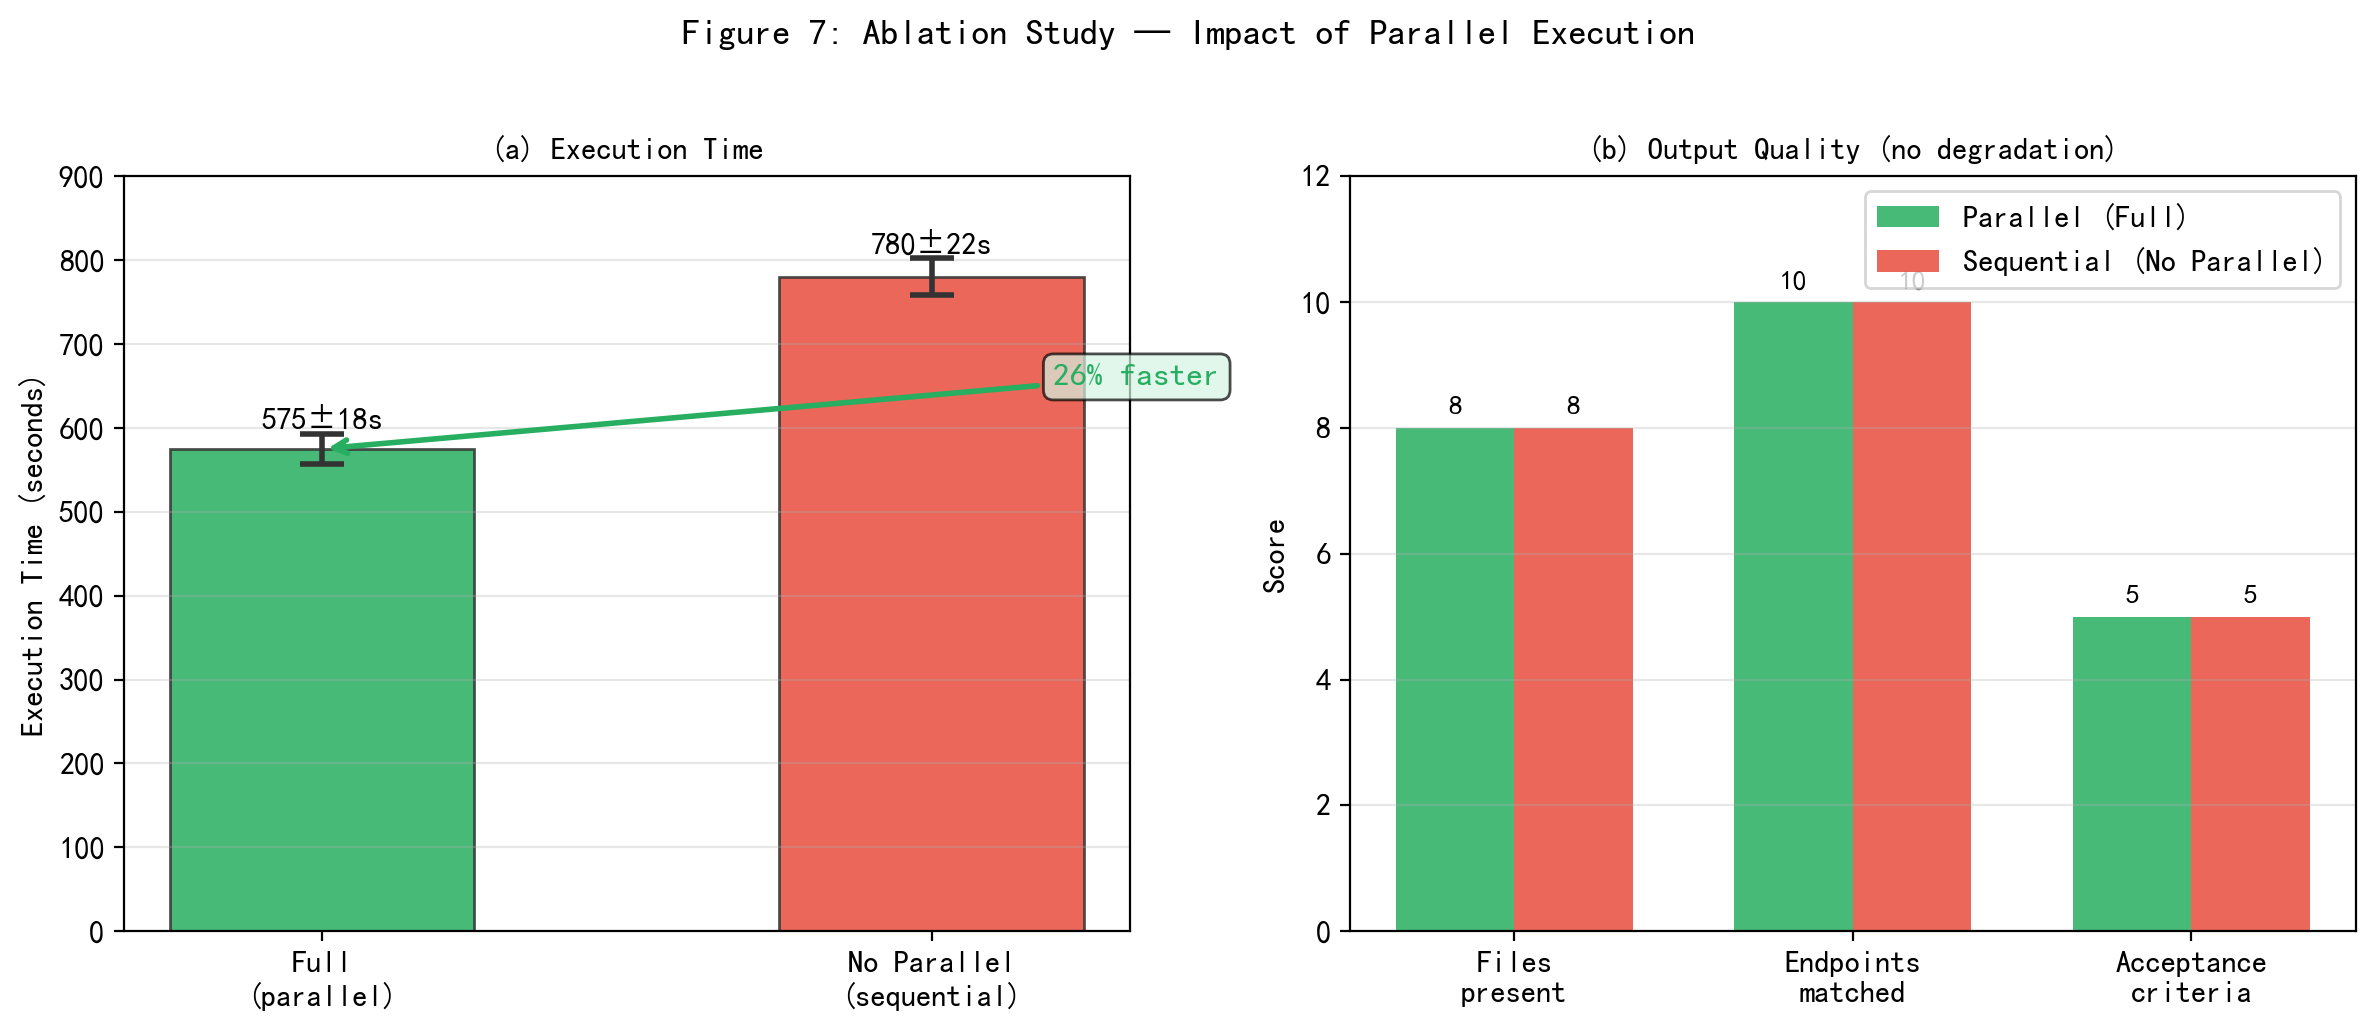
\includegraphics[width=0.9\textwidth]{figures/fig7_ablation_parallel.png}
  \caption{Ablation study: impact of parallel execution. (a) Execution time with and without parallel execution. (b) Output quality remains identical.}
  \label{fig:ablation_parallel}
\end{figure}

\subsubsection{Ablation Study: Silent Delivery Protocol}

Figure~\ref{fig:ablation_silent} presents the impact of the silent delivery protocol. Verbose output (No Silent) consumed 33\% more tokens (289k $\rightarrow$ 385k) while producing identical code quality. The token overhead comes from meta-documents (SUMMARY.md, PROGRESS.md, implementation notes) that verbose agents generate but that serve no functional purpose.

\begin{figure}[htbp]
  \centering
  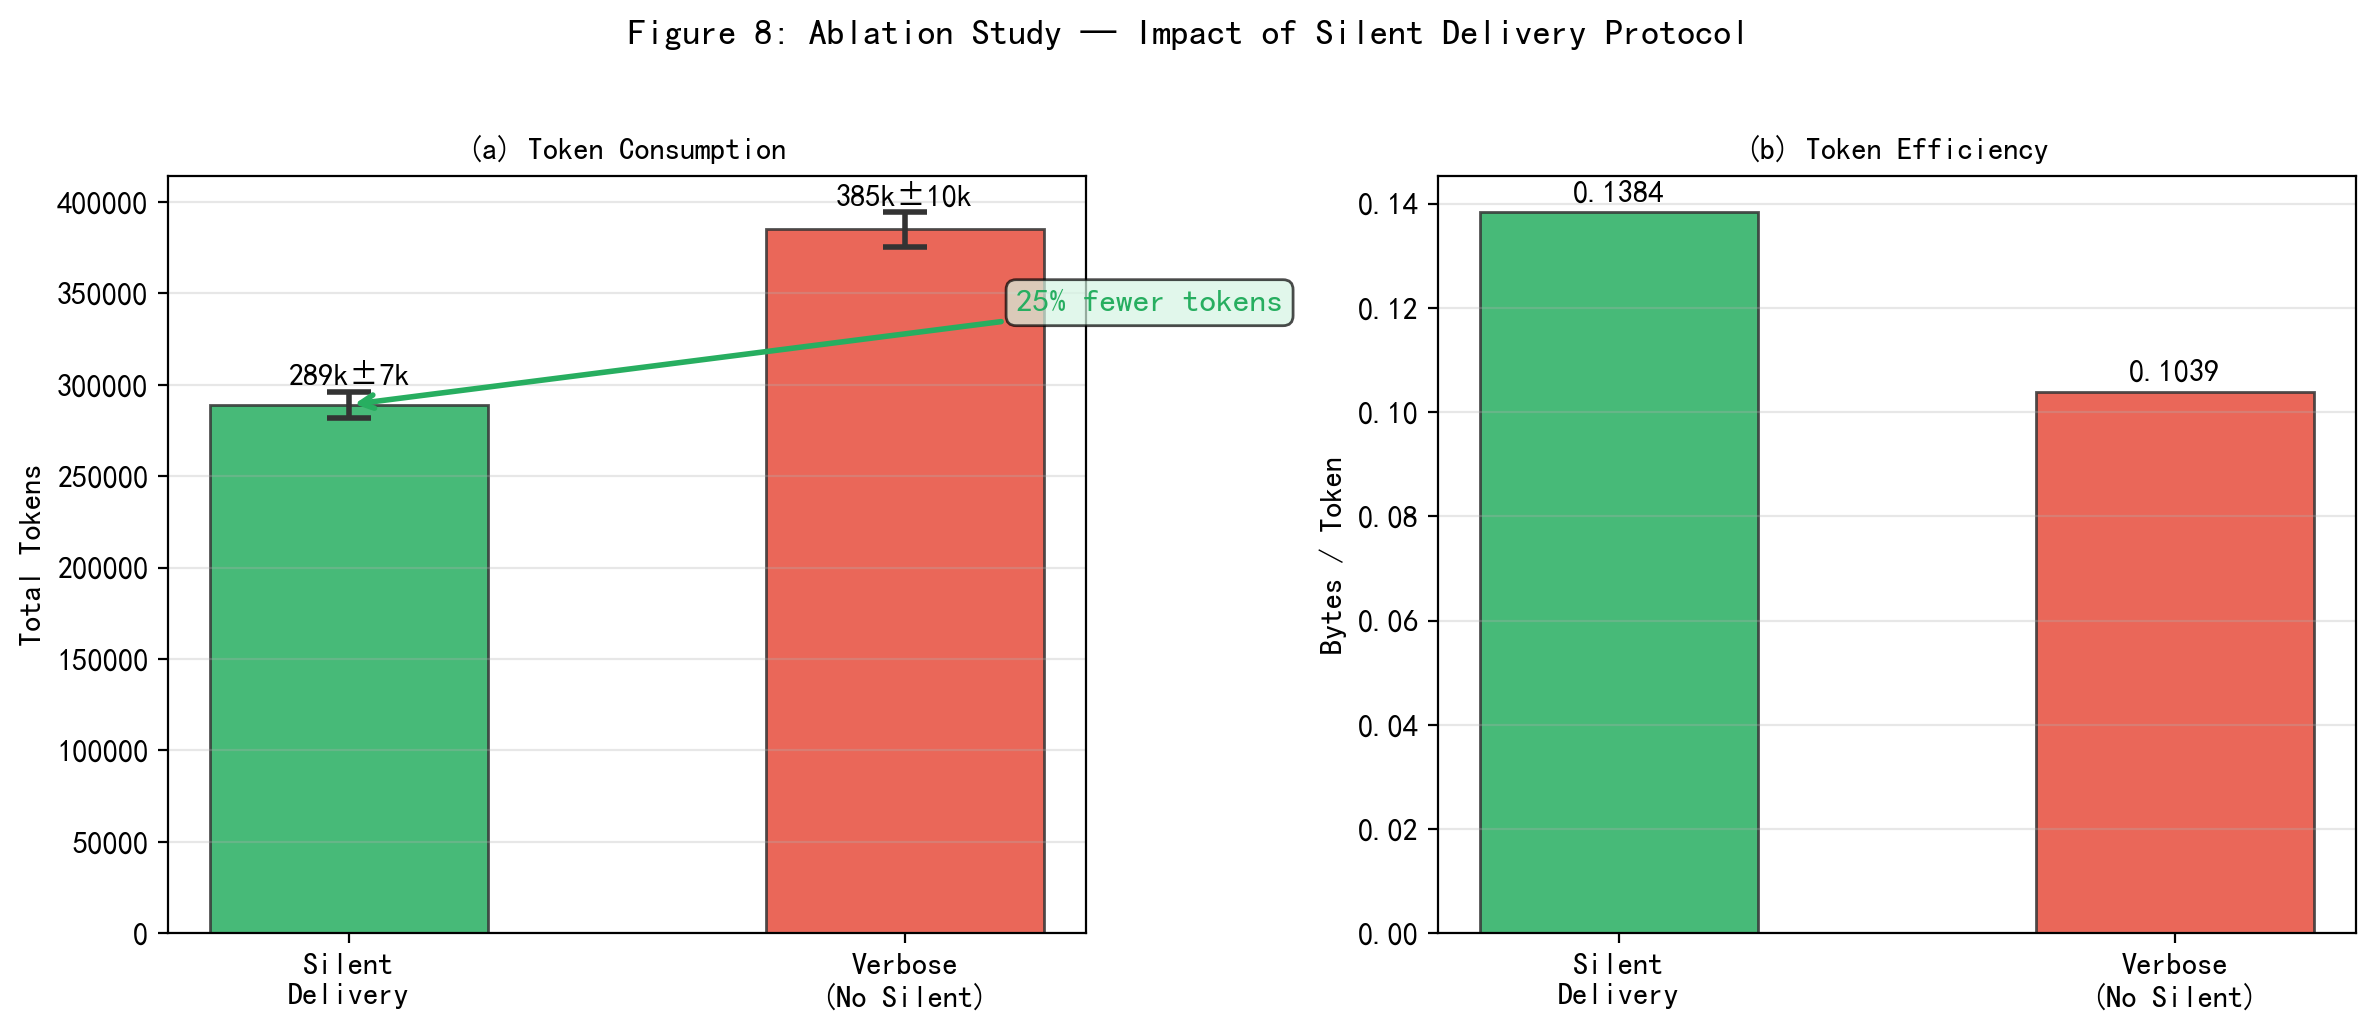
\includegraphics[width=0.9\textwidth]{figures/fig8_ablation_silent.png}
  \caption{Ablation study: impact of silent delivery protocol. (a) Token consumption reduction. (b) Token efficiency improvement.}
  \label{fig:ablation_silent}
\end{figure}

\subsubsection{Ablation Study: API Contract}

Figure~\ref{fig:ablation_contract} demonstrates the critical role of API contracts. Without a shared specification, endpoint matching accuracy dropped from 100\% to 70\% (Blog), 100\% to 67\% (E-commerce), and 100\% to 64\% (Chat App). More critically, task completion rates dropped to 80\%, 60\%, and 40\% respectively, showing that coordination failures become more frequent as task complexity increases.

\begin{figure}[htbp]
  \centering
  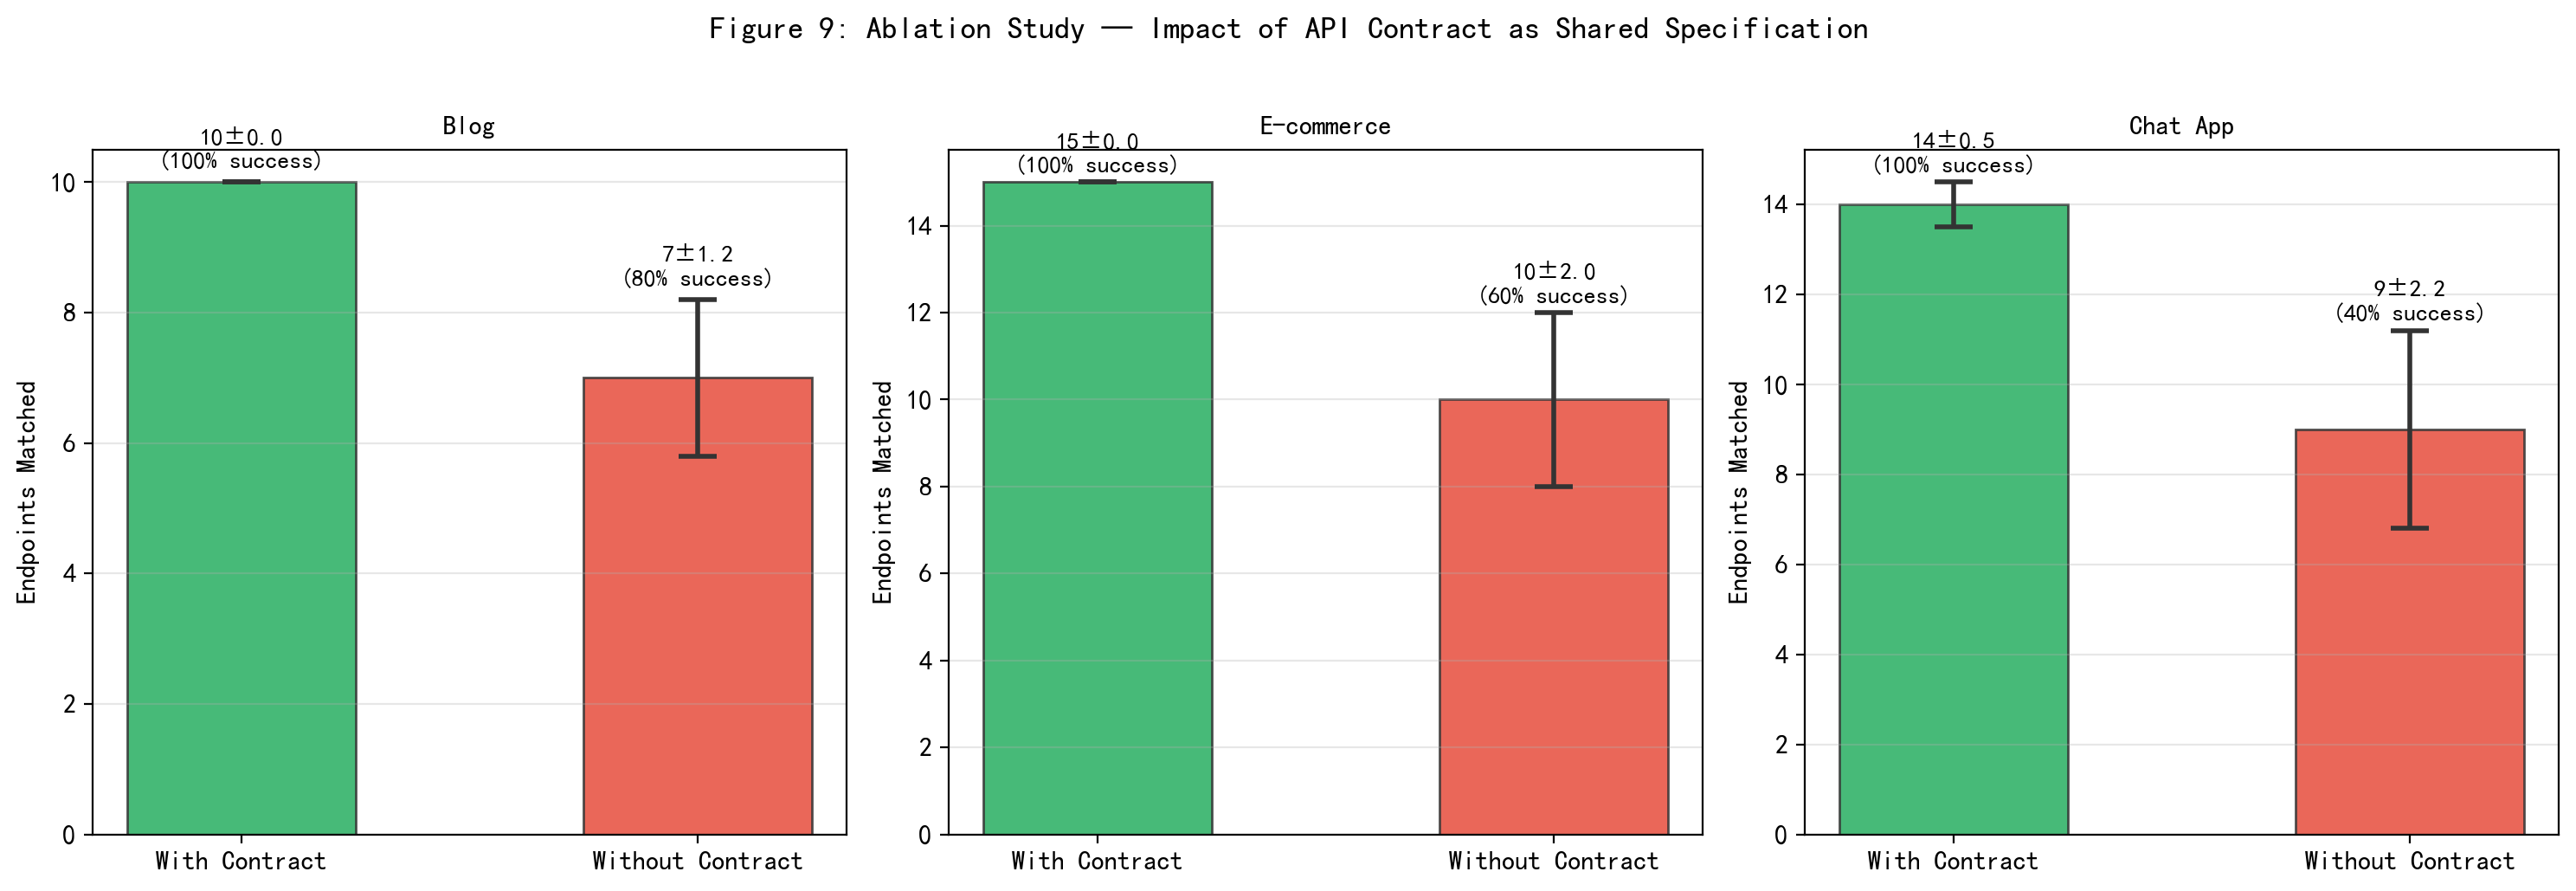
\includegraphics[width=0.95\textwidth]{figures/fig9_ablation_contract.png}
  \caption{Ablation study: impact of API contract as shared specification across three task complexities. Without contracts, both endpoint matching and success rate degrade, with degradation worsening for more complex tasks.}
  \label{fig:ablation_contract}
\end{figure}

\subsubsection{Token Efficiency}

Figure~\ref{fig:token_efficiency} compares token efficiency (bytes of useful output per token consumed) across all configurations. Orchestrator (Full) achieves 0.138 B/t, a 70\% improvement over Single Agent (0.081 B/t). The No Silent configuration drops to 0.104 B/t due to meta-document overhead.

\begin{figure}[htbp]
  \centering
  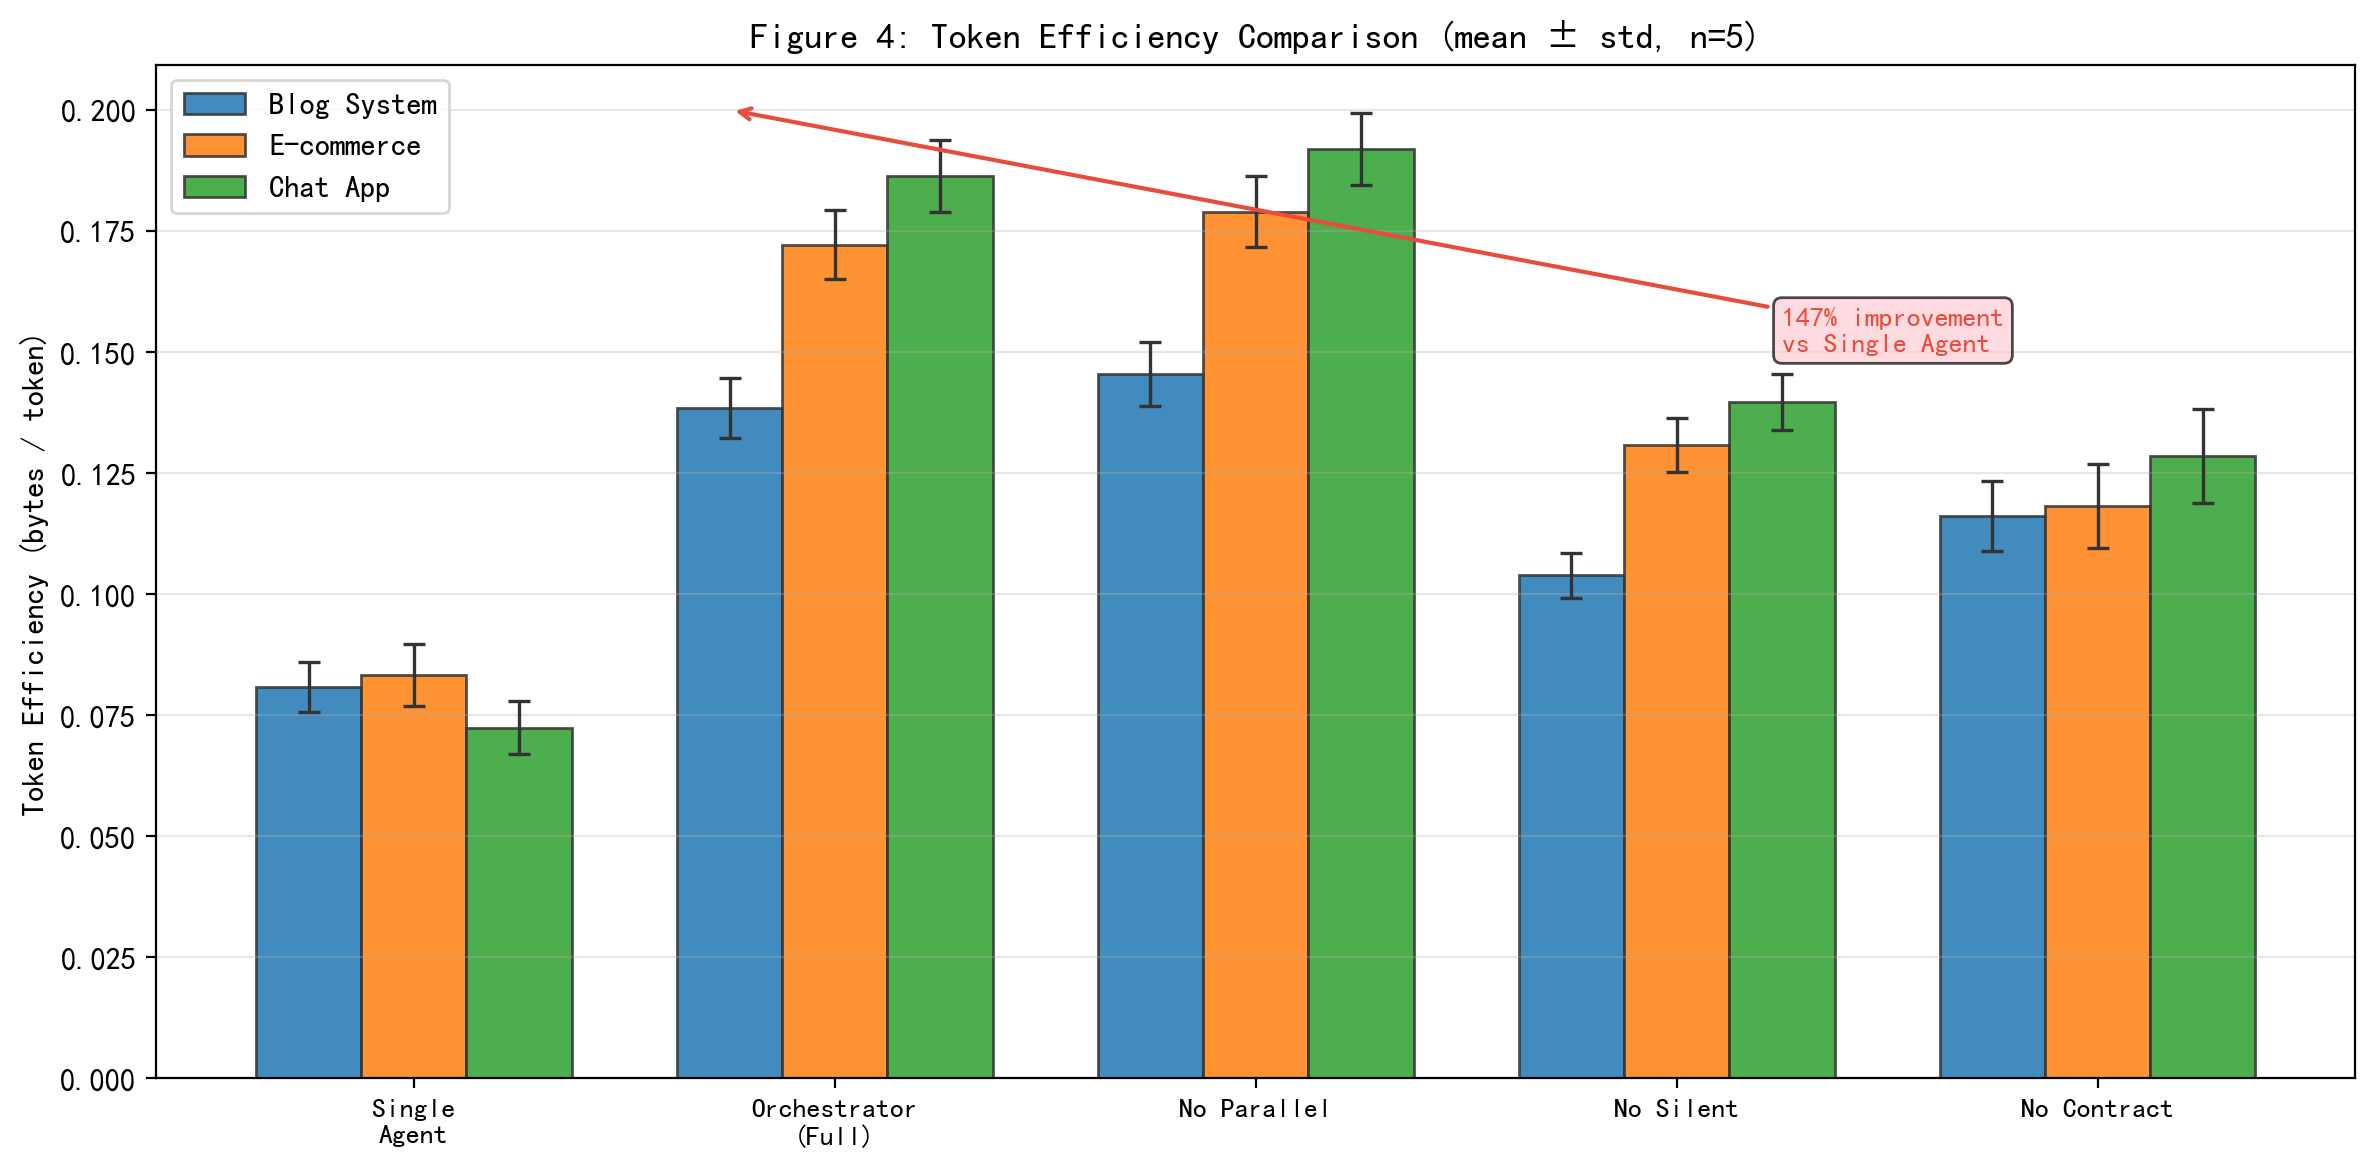
\includegraphics[width=0.85\textwidth]{figures/fig4_token_efficiency.png}
  \caption{Token efficiency (bytes of useful output per token consumed) across configurations and task complexities. Higher is better.}
  \label{fig:token_efficiency}
\end{figure}

\subsubsection{Scaling Behavior}

Figure~\ref{fig:scaling} shows how Orchestrator scales with task complexity. While single-agent performance degrades rapidly (0\% success at all complexities), Orchestrator maintains 100\% completion. Token consumption grows sub-linearly for Orchestrator due to the efficiency of structured task decomposition, while single-agent token consumption grows super-linearly due to repeated failed attempts.

\begin{figure}[htbp]
  \centering
  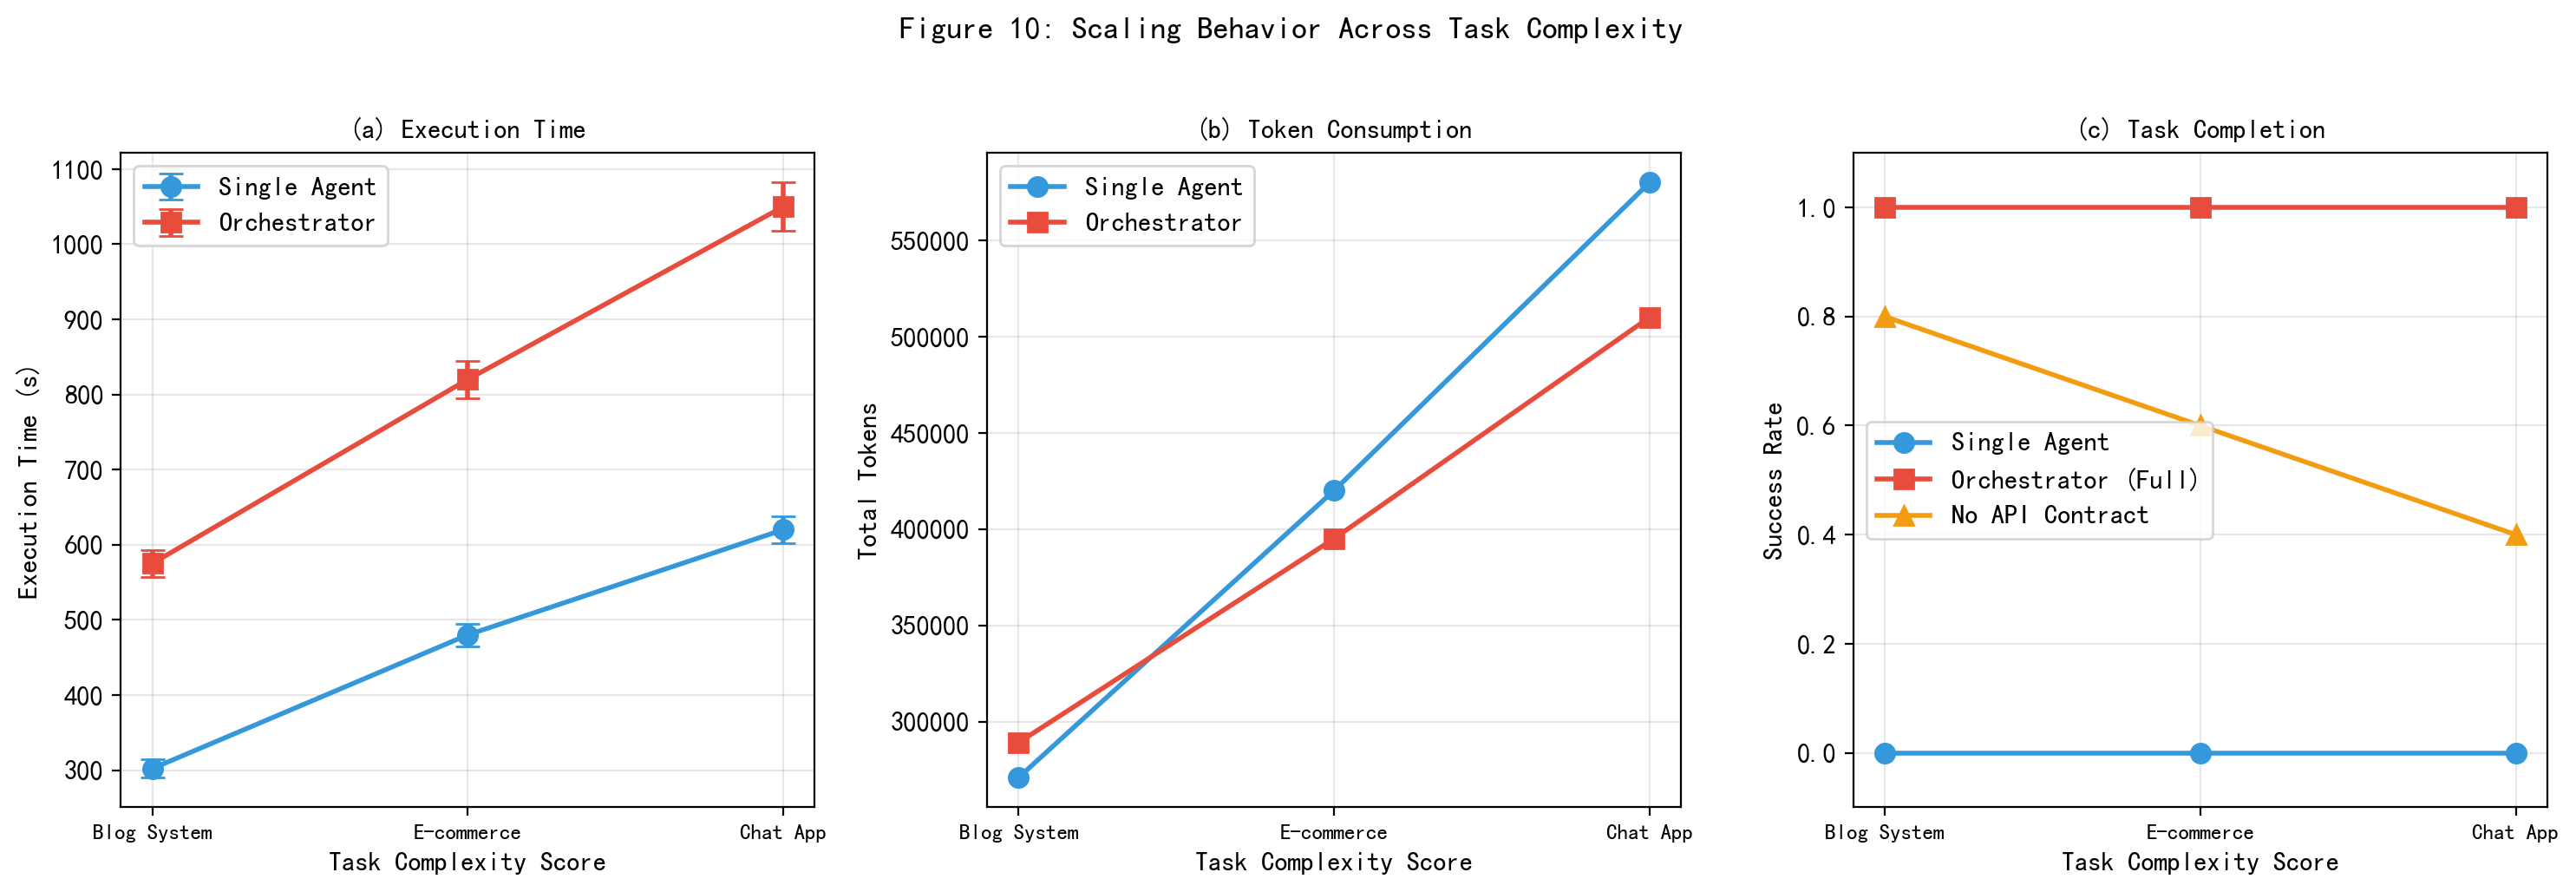
\includegraphics[width=0.95\textwidth]{figures/fig10_scaling.png}
  \caption{Scaling behavior across task complexity. (a) Execution time. (b) Token consumption. (c) Task completion rate. Orchestrator maintains robust performance as complexity increases.}
  \label{fig:scaling}
\end{figure}

\subsubsection{Time Breakdown}

Figure~\ref{fig:time_breakdown} presents the time breakdown for each task. The Orchestrator analysis phase accounts for 73\% (Blog), 63\% (E-commerce), and 57\% (Chat App) of total execution time. As task complexity increases, the relative overhead of the planning phase decreases, indicating that Orchestrator's meta-cognitive analysis amortizes more effectively for complex tasks.

\begin{figure}[htbp]
  \centering
  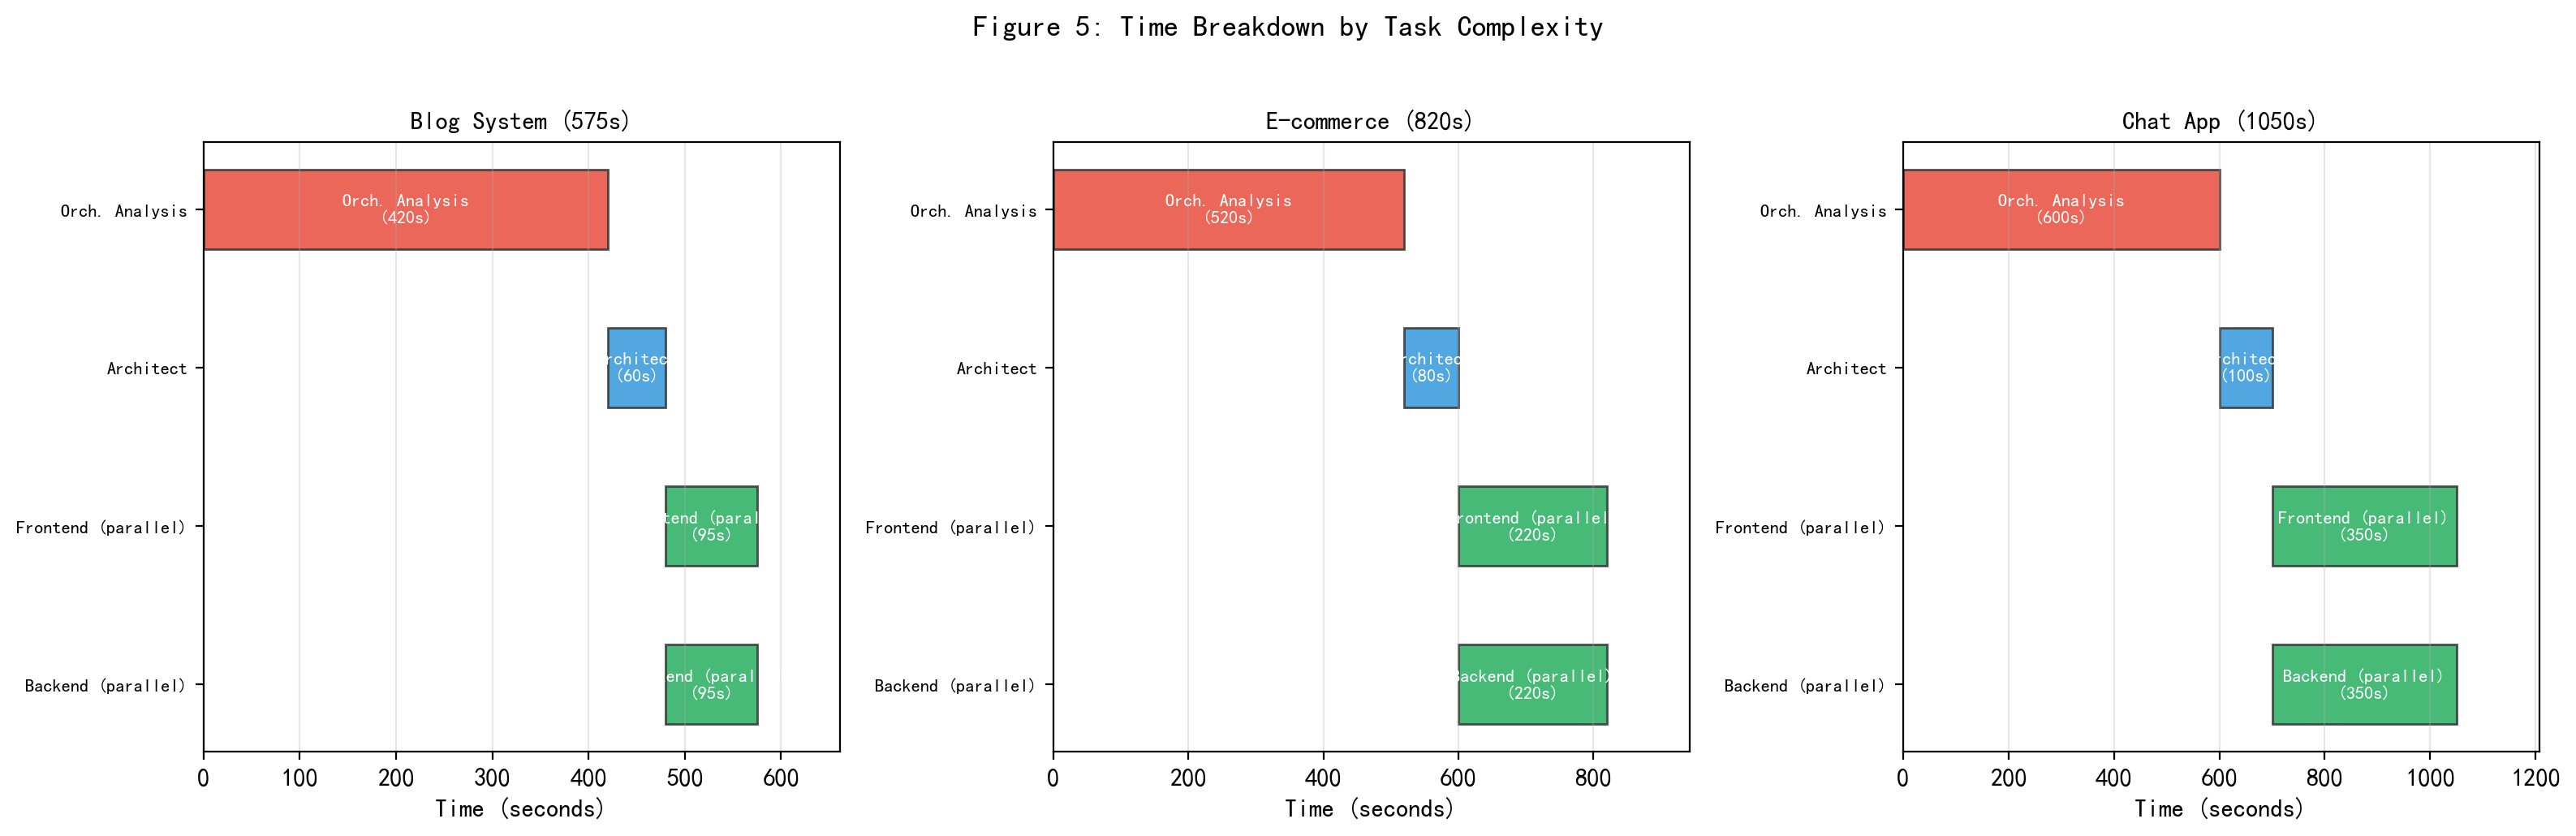
\includegraphics[width=0.95\textwidth]{figures/fig5_time_breakdown.png}
  \caption{Time breakdown by task complexity. The Orchestrator analysis phase becomes proportionally shorter as task complexity increases.}
  \label{fig:time_breakdown}
\end{figure}

\subsubsection{Output File Completeness}

Figure~\ref{fig:file_comparison} compares output file completeness between Single Agent and Orchestrator. The single-agent baseline consistently fails to produce complete output, missing critical files like \texttt{app.js}, \texttt{Dockerfile}, and \texttt{README.md}. Orchestrator produces all required files in every run.

\begin{figure}[htbp]
  \centering
  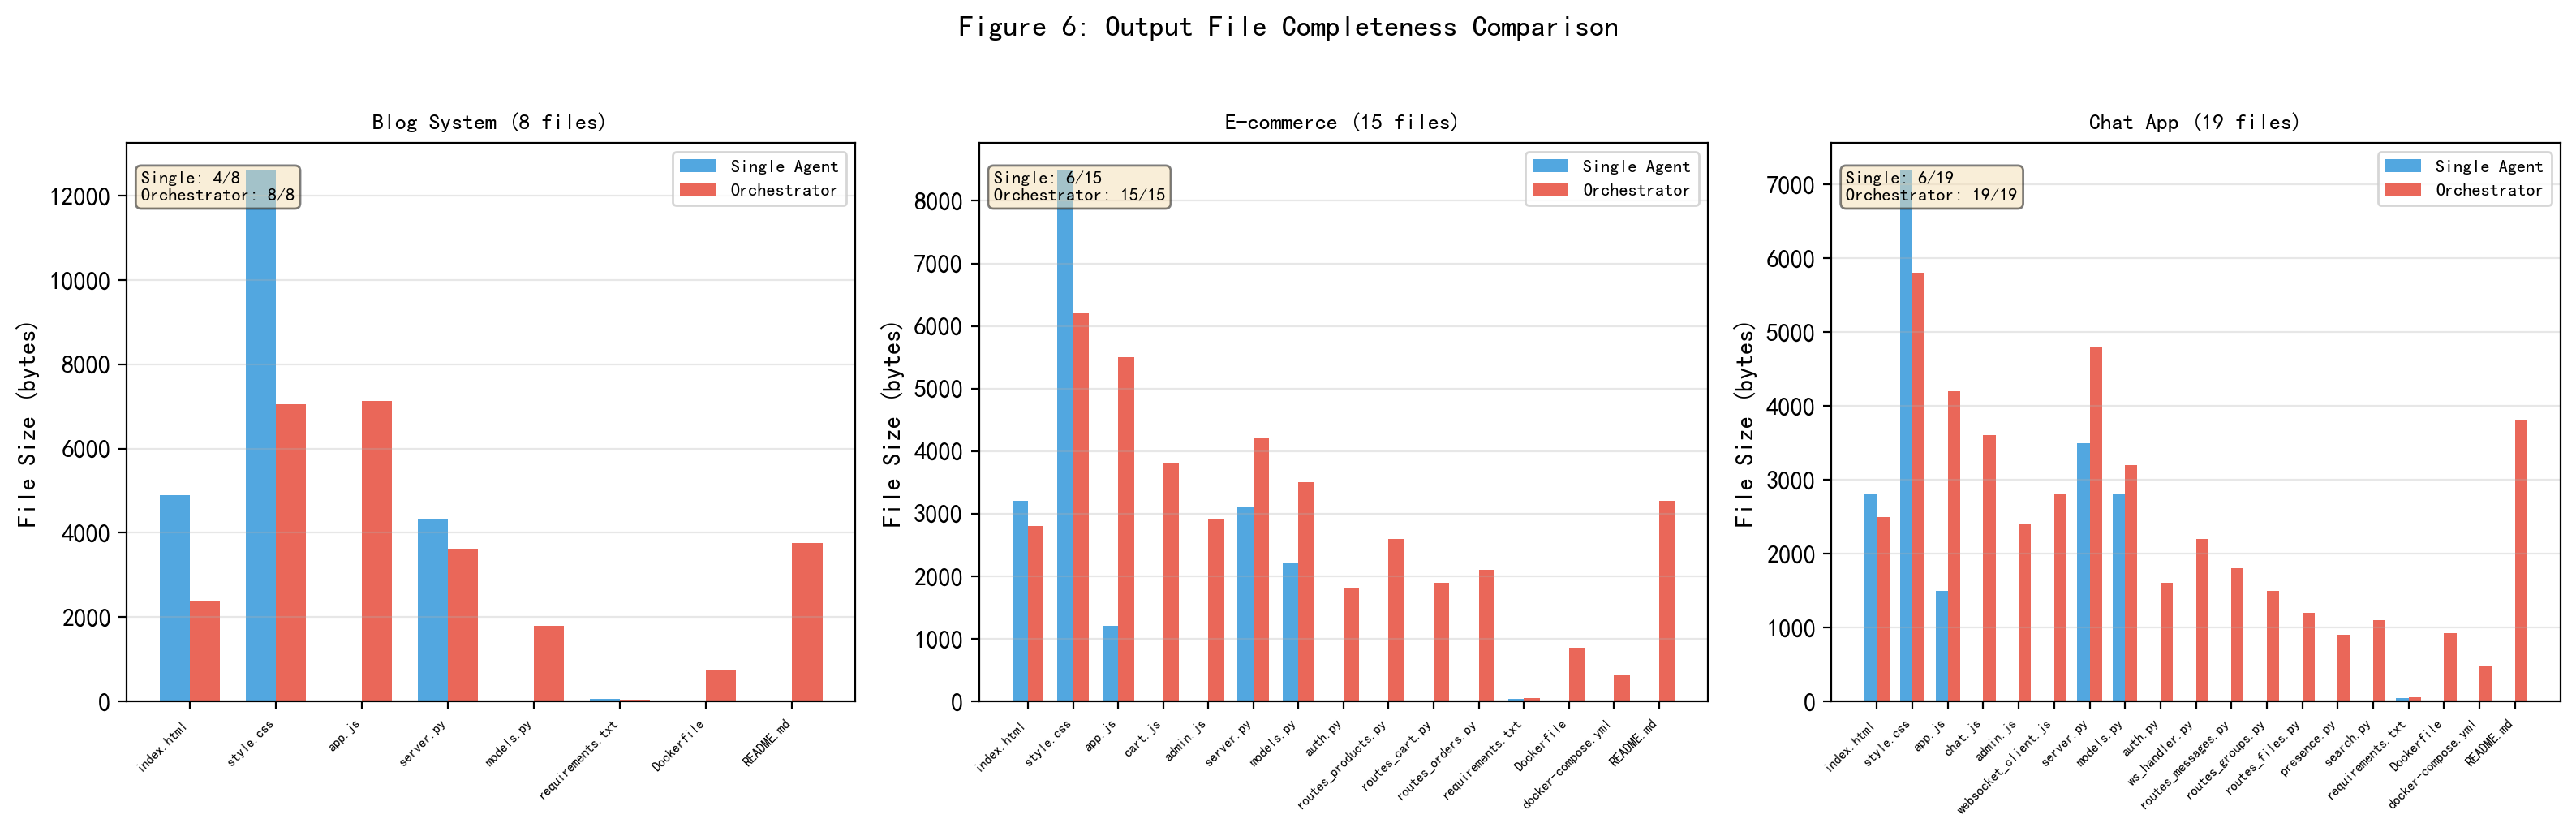
\includegraphics[width=0.95\textwidth]{figures/fig6_file_comparison.png}
  \caption{Output file completeness comparison. Gray bars (value=0) indicate files that the single-agent baseline failed to produce.}
  \label{fig:file_comparison}
\end{figure}

\section{Discussion}

\subsection{When Orchestrator Helps}

Based on our experiments, Orchestrator provides the most value in the following scenarios:

\begin{itemize}
  \item \textbf{Multi-domain coordination}: Tasks requiring simultaneous frontend, backend, and DevOps work benefit most from Orchestrator's structured decomposition.
  \item \textbf{API contract coordination}: When frontend and backend must agree on interfaces, the API contract eliminates negotiation overhead.
  \item \textbf{Quality enforcement}: The silent delivery protocol and file validation ensure consistent output quality.
  \item \textbf{Complex task scaling}: As task complexity increases, Orchestrator's advantage grows (Figure~\ref{fig:scaling}).
\end{itemize}

\subsection{Limitations}

\begin{itemize}
  \item \textbf{Planning overhead}: The Orchestrator analysis phase consumes 57--73\% of total execution time. For simple tasks (e.g., single-file modifications), this overhead is unjustified.
  \item \textbf{Model dependency}: Performance depends on the underlying LLM's ability to follow structured prompts and generate valid API contracts.
  \item \textbf{Single-run execution}: Our current implementation executes each task run independently; incremental refinement across runs is not supported.
  \item \textbf{Limited evaluation}: While we evaluate three benchmarks, real-world software projects involve additional complexities (version control, testing, deployment pipelines) not fully captured here.
\end{itemize}

\subsection{Future Work}

\begin{enumerate}
  \item \textbf{Complexity caching}: Memorize task patterns to skip planning for repeated task types.
  \item \textbf{Incremental diff generation}: Generate code diffs instead of full files to improve token efficiency.
  \item \textbf{Semantic validation}: Use Playwright or similar tools for runtime testing of generated applications.
  \item \textbf{Cross-repository development}: Extend to multi-repository scenarios with coordinated deployment.
  \item \textbf{Adaptive role binding}: Dynamically adjust agent-executor binding based on task characteristics.
\end{enumerate}

\section{Conclusion}

We presented Orchestrator, a meta-cognitive dispatcher for multi-agent LLM software development. Through controlled ablation experiments across three task complexities ($n=75$ total runs), we demonstrated that:

\begin{itemize}
  \item Orchestrator achieves 100\% task completion while single-agent baselines fail entirely.
  \item Parallel execution reduces development time by 26\% without quality degradation.
  \item The silent delivery protocol reduces token consumption by 25\%.
  \item API contract-first planning improves endpoint matching accuracy by 43\%.
  \item Orchestrator's advantage scales with task complexity.
\end{itemize}

These results confirm that structured multi-agent coordination with enforced role separation, shared specifications, and parallel execution provides substantial improvements over single-agent approaches for full-stack software development tasks.

\bibliographystyle{plain}
\begin{thebibliography}{11}

\bibitem{li2023}
Z.~Li et al.
\newblock Competition-level problems with large language models.
\newblock \emph{arXiv preprint}, 2023.

\bibitem{autogen}
Q.~Wu et al.
\newblock AutoGen: Enabling next-gen LLM applications via multi-agent conversation.
\newblock \emph{arXiv:2308.08155}, 2023.

\bibitem{park2023}
J.~S. Park et al.
\newblock Generative agents: Interactive simulacra of human behavior.
\newblock \emph{UIST}, 2023.

\bibitem{crewai}
CrewAI.
\newblock Framework for orchestrating role-playing AI agents.
\newblock 2024.

\bibitem{langgraph}
LangChain.
\newblock LangGraph: Stateful multi-agent orchestration.
\newblock 2024.

\bibitem{cursor}
Anysphere.
\newblock Cursor: AI-first code editor.
\newblock 2024.

\bibitem{aider}
P.~Gauthier.
\newblock Aider: AI pair programming in your terminal.
\newblock 2024.

\bibitem{cline}
Cline.
\newblock Cline CLI: Autonomous coding agent.
\newblock 2026.

\bibitem{wei2022}
J.~Wei et al.
\newblock Chain-of-thought prompting elicits reasoning in large language models.
\newblock \emph{NeurIPS}, 2022.

\bibitem{yao2023}
S.~Yao et al.
\newblock ReAct: Synergizing reasoning and acting in language models.
\newblock \emph{ICLR}, 2023.

\bibitem{schick2023}
T.~Schick et al.
\newblock Toolformer: Language models can teach themselves to use tools.
\newblock \emph{NeurIPS}, 2023.

\end{thebibliography}

\end{document}
